% Options for packages loaded elsewhere
\PassOptionsToPackage{unicode}{hyperref}
\PassOptionsToPackage{hyphens}{url}
%
\documentclass[
]{article}
\usepackage{amsmath,amssymb}
\usepackage{iftex}
\ifPDFTeX
  \usepackage[T1]{fontenc}
  \usepackage[utf8]{inputenc}
  \usepackage{textcomp} % provide euro and other symbols
\else % if luatex or xetex
  \usepackage{unicode-math} % this also loads fontspec
  \defaultfontfeatures{Scale=MatchLowercase}
  \defaultfontfeatures[\rmfamily]{Ligatures=TeX,Scale=1}
\fi
\usepackage{lmodern}
\ifPDFTeX\else
  % xetex/luatex font selection
\fi
% Use upquote if available, for straight quotes in verbatim environments
\IfFileExists{upquote.sty}{\usepackage{upquote}}{}
\IfFileExists{microtype.sty}{% use microtype if available
  \usepackage[]{microtype}
  \UseMicrotypeSet[protrusion]{basicmath} % disable protrusion for tt fonts
}{}
\makeatletter
\@ifundefined{KOMAClassName}{% if non-KOMA class
  \IfFileExists{parskip.sty}{%
    \usepackage{parskip}
  }{% else
    \setlength{\parindent}{0pt}
    \setlength{\parskip}{6pt plus 2pt minus 1pt}}
}{% if KOMA class
  \KOMAoptions{parskip=half}}
\makeatother
\usepackage{xcolor}
\usepackage[margin=1in]{geometry}
\usepackage{color}
\usepackage{fancyvrb}
\newcommand{\VerbBar}{|}
\newcommand{\VERB}{\Verb[commandchars=\\\{\}]}
\DefineVerbatimEnvironment{Highlighting}{Verbatim}{commandchars=\\\{\}}
% Add ',fontsize=\small' for more characters per line
\usepackage{framed}
\definecolor{shadecolor}{RGB}{248,248,248}
\newenvironment{Shaded}{\begin{snugshade}}{\end{snugshade}}
\newcommand{\AlertTok}[1]{\textcolor[rgb]{0.94,0.16,0.16}{#1}}
\newcommand{\AnnotationTok}[1]{\textcolor[rgb]{0.56,0.35,0.01}{\textbf{\textit{#1}}}}
\newcommand{\AttributeTok}[1]{\textcolor[rgb]{0.13,0.29,0.53}{#1}}
\newcommand{\BaseNTok}[1]{\textcolor[rgb]{0.00,0.00,0.81}{#1}}
\newcommand{\BuiltInTok}[1]{#1}
\newcommand{\CharTok}[1]{\textcolor[rgb]{0.31,0.60,0.02}{#1}}
\newcommand{\CommentTok}[1]{\textcolor[rgb]{0.56,0.35,0.01}{\textit{#1}}}
\newcommand{\CommentVarTok}[1]{\textcolor[rgb]{0.56,0.35,0.01}{\textbf{\textit{#1}}}}
\newcommand{\ConstantTok}[1]{\textcolor[rgb]{0.56,0.35,0.01}{#1}}
\newcommand{\ControlFlowTok}[1]{\textcolor[rgb]{0.13,0.29,0.53}{\textbf{#1}}}
\newcommand{\DataTypeTok}[1]{\textcolor[rgb]{0.13,0.29,0.53}{#1}}
\newcommand{\DecValTok}[1]{\textcolor[rgb]{0.00,0.00,0.81}{#1}}
\newcommand{\DocumentationTok}[1]{\textcolor[rgb]{0.56,0.35,0.01}{\textbf{\textit{#1}}}}
\newcommand{\ErrorTok}[1]{\textcolor[rgb]{0.64,0.00,0.00}{\textbf{#1}}}
\newcommand{\ExtensionTok}[1]{#1}
\newcommand{\FloatTok}[1]{\textcolor[rgb]{0.00,0.00,0.81}{#1}}
\newcommand{\FunctionTok}[1]{\textcolor[rgb]{0.13,0.29,0.53}{\textbf{#1}}}
\newcommand{\ImportTok}[1]{#1}
\newcommand{\InformationTok}[1]{\textcolor[rgb]{0.56,0.35,0.01}{\textbf{\textit{#1}}}}
\newcommand{\KeywordTok}[1]{\textcolor[rgb]{0.13,0.29,0.53}{\textbf{#1}}}
\newcommand{\NormalTok}[1]{#1}
\newcommand{\OperatorTok}[1]{\textcolor[rgb]{0.81,0.36,0.00}{\textbf{#1}}}
\newcommand{\OtherTok}[1]{\textcolor[rgb]{0.56,0.35,0.01}{#1}}
\newcommand{\PreprocessorTok}[1]{\textcolor[rgb]{0.56,0.35,0.01}{\textit{#1}}}
\newcommand{\RegionMarkerTok}[1]{#1}
\newcommand{\SpecialCharTok}[1]{\textcolor[rgb]{0.81,0.36,0.00}{\textbf{#1}}}
\newcommand{\SpecialStringTok}[1]{\textcolor[rgb]{0.31,0.60,0.02}{#1}}
\newcommand{\StringTok}[1]{\textcolor[rgb]{0.31,0.60,0.02}{#1}}
\newcommand{\VariableTok}[1]{\textcolor[rgb]{0.00,0.00,0.00}{#1}}
\newcommand{\VerbatimStringTok}[1]{\textcolor[rgb]{0.31,0.60,0.02}{#1}}
\newcommand{\WarningTok}[1]{\textcolor[rgb]{0.56,0.35,0.01}{\textbf{\textit{#1}}}}
\usepackage{graphicx}
\makeatletter
\newsavebox\pandoc@box
\newcommand*\pandocbounded[1]{% scales image to fit in text height/width
  \sbox\pandoc@box{#1}%
  \Gscale@div\@tempa{\textheight}{\dimexpr\ht\pandoc@box+\dp\pandoc@box\relax}%
  \Gscale@div\@tempb{\linewidth}{\wd\pandoc@box}%
  \ifdim\@tempb\p@<\@tempa\p@\let\@tempa\@tempb\fi% select the smaller of both
  \ifdim\@tempa\p@<\p@\scalebox{\@tempa}{\usebox\pandoc@box}%
  \else\usebox{\pandoc@box}%
  \fi%
}
% Set default figure placement to htbp
\def\fps@figure{htbp}
\makeatother
\setlength{\emergencystretch}{3em} % prevent overfull lines
\providecommand{\tightlist}{%
  \setlength{\itemsep}{0pt}\setlength{\parskip}{0pt}}
\setcounter{secnumdepth}{-\maxdimen} % remove section numbering
\renewcommand{\contentsname}{Índice}
\usepackage{booktabs}
\usepackage{longtable}
\usepackage{array}
\usepackage{multirow}
\usepackage{wrapfig}
\usepackage{float}
\usepackage{colortbl}
\usepackage{pdflscape}
\usepackage{tabu}
\usepackage{threeparttable}
\usepackage{threeparttablex}
\usepackage[normalem]{ulem}
\usepackage{makecell}
\usepackage{xcolor}
\usepackage{bookmark}
\IfFileExists{xurl.sty}{\usepackage{xurl}}{} % add URL line breaks if available
\urlstyle{same}
\hypersetup{
  pdftitle={ANALISIS EXPLORATORIO 1 CONCESIONARIO DE AUTOS},
  pdfauthor={Alejandra Cifuentes / Giovanny Porras},
  hidelinks,
  pdfcreator={LaTeX via pandoc}}

\title{ANALISIS EXPLORATORIO 1 CONCESIONARIO DE AUTOS}
\author{Alejandra Cifuentes / Giovanny Porras}
\date{2025-05-24}

\begin{document}
\maketitle

{
\setcounter{tocdepth}{2}
\tableofcontents
}
\subsection{2 Exploracion de datos}\label{exploracion-de-datos}

\begin{enumerate}
\def\labelenumi{\alph{enumi}.}
\tightlist
\item
  Descargar el archivo TABLA\_TALLER.xlsx
\item
  Cargar el archivo de datos en RStudio
\end{enumerate}

\textbf{Rta:} Carga de datos inicial

\begin{Shaded}
\begin{Highlighting}[]
\NormalTok{datos\_base }\OtherTok{\textless{}{-}} \FunctionTok{read\_excel}\NormalTok{(}\StringTok{"D:/MaestriaAnalitica/BasesAnalitica/gitRepository/Proyecto{-}02{-}Autos/BASE/t1fe{-}tabla\_taller.xlsx"}\NormalTok{)}
\CommentTok{\#datos\_base \textless{}{-} read\_excel("C:/Users/PC/Documents/ANALITICA/analitics01Cars/BASE/t1fe{-}tabla\_taller.xlsx")}
\FunctionTok{kable}\NormalTok{(}\FunctionTok{head}\NormalTok{(datos\_base, }\DecValTok{10}\NormalTok{,  }\AttributeTok{caption =} \StringTok{"Datos iniciales"}\NormalTok{), }\AttributeTok{format =} \StringTok{"latex"}\NormalTok{, }\AttributeTok{booktabs =} \ConstantTok{TRUE}\NormalTok{) }\SpecialCharTok{\%\textgreater{}\%} 
  \FunctionTok{kable\_styling}\NormalTok{(}\AttributeTok{latex\_options =} \FunctionTok{c}\NormalTok{(}\StringTok{"scale\_down"}\NormalTok{, }\StringTok{"hold\_position"}\NormalTok{))}
\end{Highlighting}
\end{Shaded}

\begin{table}[!h]
\centering
\resizebox{\ifdim\width>\linewidth\linewidth\else\width\fi}{!}{
\begin{tabular}{lllllllrl}
\toprule
PERSONA & EDAD & SEXO & ESTATURA & NIVEL ESCOLAR & MARCA DE AUTO & NUMERO DE HIJOS & SALARIO & MASCOTA\\
\midrule
NA & NA & NA & NA & NA & NA & NA & NA & NA\\
NA & NA & NA & NA & NA & NA & NA & NA & NA\\
PERSONA 1 & 21 & M & 1.54 & MAESTRÍA & AUDI & 0 & 1200000 & SI\\
PERSONA 2 & 26 & F & 1.55 & PROFESIONAL & RENAULT & 5 & 1250000 & NO\\
PERSONA 3 & 30 & F & 1.6 & DOCTORADO & BMW & 2 & 900000 & NO\\
\addlinespace
PERSONA 4 & 31 & f & 1.7 & PROFESIONAL & RENAULT & 2 & 800000 & NO\\
PERSONA 5 & 35 & M & 1.71 & MAESTRÍA & AUDI & 1 & 950000 & NO\\
PERSONA 6 & 65 & M & 1.8 & MAESTRÍA & AUDI & 1 & 2000000 & SI\\
PERSONA 7 & 45 & M & 1.54 & MAESTRÍA & BMW & 1 & 2500000 & NO\\
PERSONA 8 & 42 & F & 1.52 & PROFESIONAL & RENAULT & 1 & 3500000 & SI\\
\bottomrule
\end{tabular}}
\end{table}

\begin{enumerate}
\def\labelenumi{\alph{enumi}.}
\setcounter{enumi}{2}
\tightlist
\item
  Describir brevemente la estructura del conjunto de datos: ¿Cuantos
  clientes estan registrados y que variables incluyen?
\end{enumerate}

\begin{Shaded}
\begin{Highlighting}[]
\NormalTok{no\_datos\_persona }\OtherTok{\textless{}{-}}\NormalTok{ datos\_base }\SpecialCharTok{\%\textgreater{}\%}
  \FunctionTok{filter}\NormalTok{(}\FunctionTok{grepl}\NormalTok{(}\StringTok{"PERSONA"}\NormalTok{, PERSONA)) }\SpecialCharTok{\%\textgreater{}\%}
  \FunctionTok{count}\NormalTok{()}

\NormalTok{cabeceras\_datos }\OtherTok{\textless{}{-}} \FunctionTok{names}\NormalTok{(datos\_base)}
\end{Highlighting}
\end{Shaded}

\textbf{Rta:} El conjunto de datos tiene 60 clientes registrados e
incluyen las varibles PERSONA, EDAD, SEXO, ESTATURA, NIVEL ESCOLAR,
MARCA DE AUTO, NUMERO DE HIJOS, SALARIO, MASCOTA .

\begin{enumerate}
\def\labelenumi{\alph{enumi}.}
\setcounter{enumi}{3}
\tightlist
\item
  Realizar una exploracion rapida utilizando funciones como head(),
  tail(), str(), summary(), \textbf{Rta:} Los ultimos valores son (tail)
\end{enumerate}

\begin{Shaded}
\begin{Highlighting}[]
\NormalTok{ultimos\_datos }\OtherTok{\textless{}{-}} \FunctionTok{tail}\NormalTok{(datos\_base)}
\FunctionTok{kable}\NormalTok{(}\FunctionTok{head}\NormalTok{(ultimos\_datos, }\DecValTok{10}\NormalTok{, }\AttributeTok{caption =} \StringTok{"Datos ultima posicion"}\NormalTok{), }\AttributeTok{format =} \StringTok{"latex"}\NormalTok{, }\AttributeTok{booktabs =} \ConstantTok{TRUE}\NormalTok{) }\SpecialCharTok{\%\textgreater{}\%}\FunctionTok{kable\_styling}\NormalTok{(}\AttributeTok{latex\_options =} \FunctionTok{c}\NormalTok{(}\StringTok{"scale\_down"}\NormalTok{, }\StringTok{"hold\_position"}\NormalTok{))}
\end{Highlighting}
\end{Shaded}

\begin{table}[!h]
\centering
\resizebox{\ifdim\width>\linewidth\linewidth\else\width\fi}{!}{
\begin{tabular}{lllllllrl}
\toprule
PERSONA & EDAD & SEXO & ESTATURA & NIVEL ESCOLAR & MARCA DE AUTO & NUMERO DE HIJOS & SALARIO & MASCOTA\\
\midrule
PERSONA 55 & 30 & F & 1.54 & MAESTRÍA & CHEVROLET & 2 & 2400000 & SI\\
PERSONA 56 & 39 & M & 1.58 & MAESTRÍA & AUDI & 1 & 2600000 & NO\\
PERSONA 57 & 34 & F & 1.6 & DOCTORADO & BMW & 1 & 3500000 & SI\\
PERSONA 58 & 24 & f & 1.7 & PROFESIONAL & RENAULT & 3 & 800000 & SI\\
PERSONA 59 & 20 & M & 1.71 & MAESTRÍA & AUDI & 0 & 850000 & NO\\
\addlinespace
PERSONA 60 & 10 & M & 1.8 & PROFESIONAL & AUDI & 0 & 1000000 & NO\\
\bottomrule
\end{tabular}}
\end{table}

\textbf{Funciones adicionales:}

\begin{Shaded}
\begin{Highlighting}[]
\CommentTok{\#print(str(datos\_base))}
\CommentTok{\#print(dim(datos\_base))}
\CommentTok{\#print(colnames(datos\_base))}
\FunctionTok{print}\NormalTok{(}\FunctionTok{summary}\NormalTok{(datos\_base))}
\end{Highlighting}
\end{Shaded}

\begin{verbatim}
##    PERSONA              EDAD               SEXO             ESTATURA        
##  Length:62          Length:62          Length:62          Length:62         
##  Class :character   Class :character   Class :character   Class :character  
##  Mode  :character   Mode  :character   Mode  :character   Mode  :character  
##                                                                             
##                                                                             
##                                                                             
##                                                                             
##  NIVEL ESCOLAR      MARCA DE AUTO      NUMERO DE HIJOS       SALARIO       
##  Length:62          Length:62          Length:62          Min.   : 800000  
##  Class :character   Class :character   Class :character   1st Qu.:2000000  
##  Mode  :character   Mode  :character   Mode  :character   Median :3450000  
##                                                           Mean   :3286667  
##                                                           3rd Qu.:4700000  
##                                                           Max.   :6500000  
##                                                           NA's   :2        
##    MASCOTA         
##  Length:62         
##  Class :character  
##  Mode  :character  
##                    
##                    
##                    
## 
\end{verbatim}

\begin{enumerate}
\def\labelenumi{\alph{enumi}.}
\setcounter{enumi}{4}
\tightlist
\item
  Identificar si hay datos faltantes y cuantificar cuantos son en total
  y por variable
\end{enumerate}

\begin{Shaded}
\begin{Highlighting}[]
\CommentTok{\#is.na(datos\_base)}
\NormalTok{total\_na }\OtherTok{=}\NormalTok{ datos\_base }\SpecialCharTok{\%\textgreater{}\%}\NormalTok{ is.na }\SpecialCharTok{\%\textgreater{}\%} \FunctionTok{sum}\NormalTok{()  }
\CommentTok{\#Contar NA por columna(variable) }
\NormalTok{na\_por\_columna }\OtherTok{\textless{}{-}} \FunctionTok{colSums}\NormalTok{(}\FunctionTok{is.na}\NormalTok{(datos\_base))}
\NormalTok{tabla\_na }\OtherTok{\textless{}{-}} \FunctionTok{data.frame}\NormalTok{(}
   \AttributeTok{Variable =} \FunctionTok{names}\NormalTok{(na\_por\_columna), }
   \AttributeTok{total\_na =} \FunctionTok{as.vector}\NormalTok{(na\_por\_columna) }
\NormalTok{)}

\CommentTok{\#Contar NA total }
\CommentTok{\#rowSums(is.na(datos\_base))}

\CommentTok{\#Impresion de tabla }
\CommentTok{\#kable(tabla\_na, caption = "Variables faltantes por cuantificar")  \%\textgreater{}\%}
\CommentTok{\#  kable\_styling(full\_width = FALSE, position = "left")}
\end{Highlighting}
\end{Shaded}

\textbf{Rta}: - El numero de total de datos faltantes es \textbf{24} y
por variable son los siguientes:

\begin{longtable}[l]{lr}
\caption{\label{tab:tabla_variables_na}Variables faltantes por cuantificar}\\
\toprule
Variable & total\_na\\
\midrule
PERSONA & 2\\
EDAD & 2\\
SEXO & 3\\
ESTATURA & 2\\
NIVEL ESCOLAR & 3\\
\addlinespace
MARCA DE AUTO & 4\\
NUMERO DE HIJOS & 3\\
SALARIO & 2\\
MASCOTA & 3\\
\bottomrule
\end{longtable}

\begin{itemize}
\tightlist
\item
  Analisis: Hay problemas de datos en todas las variables sera
  importante discriminar cada caso
\end{itemize}

\begin{enumerate}
\def\labelenumi{\alph{enumi}.}
\setcounter{enumi}{5}
\tightlist
\item
  Comentar sobre los posibles problemas en los datos:
\end{enumerate}

\textbf{Filas vacías al inicio del archivo:} - Las dos primeras filas
están vacías o no contienen datos válidos.

\textbf{Inconsistencias categóricas:}

\begin{itemize}
\tightlist
\item
  Variabilidad en la codificación de la variable SEXO, con valores como
  f, mujer, hombre, nan o minúsculas inconsistentes.
\item
  Formatos no estandarizados en NIVEL ESCOLAR, como el uso de PhD en
  lugar de DOCTORADO.
\item
  Uso de minúsculas en valores de MARCA DE AUTO, como renault.
\end{itemize}

\textbf{Valores faltantes:}

\begin{itemize}
\tightlist
\item
  Algunas filas tienen múltiples variables vacías, como en el caso de la
  PERSONA 24.
\end{itemize}

\textbf{Valores extremos o anómalos (outliers):}

\begin{itemize}
\tightlist
\item
  PERSONA 31: valor de ESTATURA = 3.45 m, fuera del rango fisiológico
  normal.
\item
  PERSONA 33: valor de NUMERO DE HIJOS = 54, ampliamente fuera del
  promedio observado (3.03).
\end{itemize}

\newpage

\subsection{3 Análisis de la variable Marca ``Marca de
auto''.}\label{anuxe1lisis-de-la-variable-marca-marca-de-auto.}

\begin{enumerate}
\def\labelenumi{\alph{enumi}.}
\tightlist
\item
  Evaluar la variable \textbf{``MARCA DE AUTO''} y determinar si hay
  faltantes.
\end{enumerate}

\begin{Shaded}
\begin{Highlighting}[]
\NormalTok{ data\_na\_marca\_autos }\OtherTok{\textless{}{-}} \FunctionTok{sum}\NormalTok{(}\FunctionTok{is.na}\NormalTok{(datos\_base}\SpecialCharTok{$}\StringTok{\textasciigrave{}}\AttributeTok{MARCA DE AUTO}\StringTok{\textasciigrave{}}\NormalTok{))}
\end{Highlighting}
\end{Shaded}

\textbf{Rta:} Se tratan datos faltantes y se encuentran un total de
\textbf{4}; se realiza tratamiento de datos remplazando los
``na''/``NA'' a ``SIN\_CONFIRMAR'', se convierte todo mayúsculas.

\begin{Shaded}
\begin{Highlighting}[]
 \CommentTok{\#Tratamiento datos MARCA DE AUTOS }
 \CommentTok{\#Eliminar columna 1, 2 }
\NormalTok{ datos\_base }\OtherTok{\textless{}{-}}\NormalTok{ datos\_base[}\SpecialCharTok{{-}}\FunctionTok{c}\NormalTok{(}\DecValTok{1}\NormalTok{,}\DecValTok{2}\NormalTok{), ]}
 \CommentTok{\#Datos Eliminados}
\NormalTok{ na\_marca\_autos }\OtherTok{\textless{}{-}} \FunctionTok{sum}\NormalTok{(}\FunctionTok{is.na}\NormalTok{(datos\_base}\SpecialCharTok{$}\StringTok{\textasciigrave{}}\AttributeTok{MARCA DE AUTO}\StringTok{\textasciigrave{}}\NormalTok{)) }
 \CommentTok{\# PERSONA 13, 32, 49, NA y datos vacios }
\NormalTok{ datos\_base}\SpecialCharTok{$}\StringTok{\textasciigrave{}}\AttributeTok{MARCA DE AUTO}\StringTok{\textasciigrave{}}\NormalTok{[}\FunctionTok{is.na}\NormalTok{(datos\_base}\SpecialCharTok{$}\StringTok{\textasciigrave{}}\AttributeTok{MARCA DE AUTO}\StringTok{\textasciigrave{}}\NormalTok{) }\SpecialCharTok{|}\NormalTok{ datos\_base}\SpecialCharTok{$}\StringTok{\textasciigrave{}}\AttributeTok{MARCA DE AUTO}\StringTok{\textasciigrave{}} \SpecialCharTok{==} \StringTok{"NA"}\NormalTok{] }\OtherTok{\textless{}{-}} \StringTok{"SIN\_CONFIRMAR"}
 \CommentTok{\# PERSONA 39 cambia FOR A FORD }
\NormalTok{ datos\_base}\SpecialCharTok{$}\StringTok{\textasciigrave{}}\AttributeTok{MARCA DE AUTO}\StringTok{\textasciigrave{}}\NormalTok{[ datos\_base}\SpecialCharTok{$}\StringTok{\textasciigrave{}}\AttributeTok{MARCA DE AUTO}\StringTok{\textasciigrave{}} \SpecialCharTok{==} \StringTok{"FOR"}\NormalTok{] }\OtherTok{\textless{}{-}} \StringTok{"FORD"}
 \CommentTok{\# PERSONA 40 cambia BWM A BMW }
\NormalTok{ datos\_base}\SpecialCharTok{$}\StringTok{\textasciigrave{}}\AttributeTok{MARCA DE AUTO}\StringTok{\textasciigrave{}}\NormalTok{[ datos\_base}\SpecialCharTok{$}\StringTok{\textasciigrave{}}\AttributeTok{MARCA DE AUTO}\StringTok{\textasciigrave{}} \SpecialCharTok{==} \StringTok{"BWM"}\NormalTok{] }\OtherTok{\textless{}{-}} \StringTok{"BMW"}
 \CommentTok{\# PERSONA 36 cambio a mayuscula marca }
\NormalTok{ datos\_base}\SpecialCharTok{$}\StringTok{\textasciigrave{}}\AttributeTok{MARCA DE AUTO}\StringTok{\textasciigrave{}} \OtherTok{\textless{}{-}} \FunctionTok{toupper}\NormalTok{(datos\_base}\SpecialCharTok{$}\StringTok{\textasciigrave{}}\AttributeTok{MARCA DE AUTO}\StringTok{\textasciigrave{}}\NormalTok{)}
\end{Highlighting}
\end{Shaded}

\begin{enumerate}
\def\labelenumi{\alph{enumi}.}
\setcounter{enumi}{1}
\tightlist
\item
  Crear una tabla de frecuencias para entender la popularidad de las
  diferentes marcas entre los cliente.
\end{enumerate}

\textbf{Rta: }En la tabla de frecuencias se observa que las marcas más
populares son AUDI, CHEVROLET, RENAULT y BMW. Los tres usuarios que no
tienen la categoría ``\,``SIN\_CONFIRMAR''\,'' se identificaron como
personas a partir de 50 años.

\begin{tabular}{lr}
\toprule
MARCA DE AUTO & Frecuencia\\
\midrule
AUDI & 13\\
RENAULT & 13\\
BMW & 12\\
CHEVROLET & 12\\
FORD & 7\\
\addlinespace
SIN\_CONFIRMAR & 3\\
\bottomrule
\end{tabular}

\begin{enumerate}
\def\labelenumi{\alph{enumi}.}
\setcounter{enumi}{2}
\tightlist
\item
  Generar gráficos de barras y de tortas para visualizar la distribución
  de las marcas de autos y proporcionar una interpretación.
\end{enumerate}

\textbf{Rta: } - Se identifica que las marcas de vehículos preferidas
por los clientes del concesionario son \textbf{AUDI} y \textbf{RENAULT};
se observa una segmentación igual por pares entre las entre AUDI/RENAULT
y CHEVROLET/BMW

\begin{itemize}
\tightlist
\item
  La preferencia de vehículos esta distribuida entre 4 marcas que suman
  83\% de la muestra, estas cuatro marcas a su vez representan dos
  segmentos que se reparten en el mismo porcentaje 21\%/21\% y
  20\%/20\%.
\end{itemize}

\begin{Shaded}
\begin{Highlighting}[]
\NormalTok{ grafico\_barras }\SpecialCharTok{+}\NormalTok{ grafico\_pastel   }\SpecialCharTok{+} \FunctionTok{plot\_layout}\NormalTok{(}\AttributeTok{widths =} \FunctionTok{c}\NormalTok{(}\DecValTok{4}\NormalTok{, }\FloatTok{4.5}\NormalTok{))}
\end{Highlighting}
\end{Shaded}

\pandocbounded{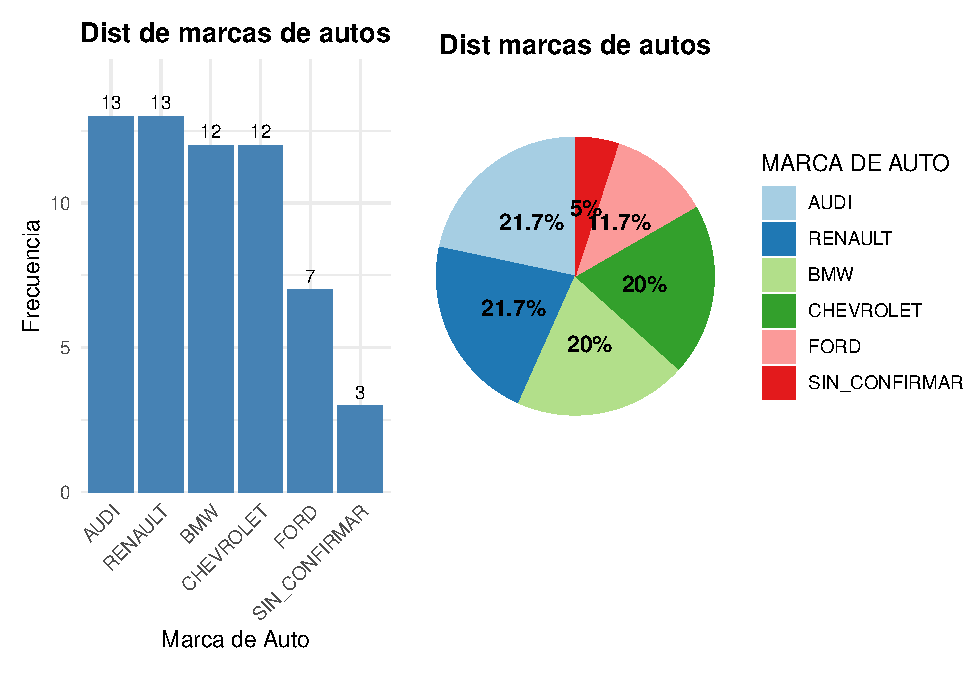
\includegraphics[keepaspectratio]{Reporte01-autors_files/figure-latex/unnamed-chunk-4-1.pdf}}

\begin{enumerate}
\def\labelenumi{\alph{enumi}.}
\setcounter{enumi}{3}
\tightlist
\item
  Concluir cuál es la marca de auto más popular entre los clientes.
\end{enumerate}

\textbf{Rta: } Se concluyen que AUDI y RENAULT son las marcas lideres
con una distribución uniforme en el los clientes del concesionario en un
porcentaje del 21.7 entre ambas ocupan el 42.4\%.

\newpage

\subsection{4 Análisis de la variable
``Edad''.}\label{anuxe1lisis-de-la-variable-edad.}

\begin{enumerate}
\def\labelenumi{\alph{enumi}.}
\tightlist
\item
  Verificar si la variable ``EDAD'' está correctamente importada como
  tipo numérico.
\end{enumerate}

\textbf{Rta:} La variable edad es de tipo \textbf{caracter} sin embargo
su naturaleza es de tipo Cuantitativa discreta para este conjunto de
datos por este motivo se va a relizar la conversión a \textbf{numeric}
en la sección dedicada a normalización de datos.

\begin{Shaded}
\begin{Highlighting}[]
\FunctionTok{summary}\NormalTok{(datos\_base}\SpecialCharTok{$}\NormalTok{EDAD)}
\end{Highlighting}
\end{Shaded}

\begin{verbatim}
##    Length     Class      Mode 
##        60 character character
\end{verbatim}

\begin{enumerate}
\def\labelenumi{\alph{enumi}.}
\setcounter{enumi}{1}
\tightlist
\item
  Identificar cualquier valor incorrecto (por ejemplo, texto en lugar de
  números) y corrija los errores.
\end{enumerate}

\textbf{Rta: }Se encuentran datos incosistententes por formato y
\textbf{NA} se imputa la media para ambos casos, para el caso de
aoutfillers se trabaja con el datos atipico de 10 años para la persona
que tenia una edad de 10 años imputando la media.

\begin{Shaded}
\begin{Highlighting}[]
\CommentTok{\#TRATAMIENTO DE DATOS EDAD }
\CommentTok{\#Agrega NA a los datos que no se pueden convertir a numerico }
\NormalTok{datos\_base}\SpecialCharTok{$}\NormalTok{EDAD }\OtherTok{\textless{}{-}} \FunctionTok{as.numeric}\NormalTok{(datos\_base}\SpecialCharTok{$}\NormalTok{EDAD)}
\end{Highlighting}
\end{Shaded}

\begin{verbatim}
## Warning: NAs introducidos por coerción
\end{verbatim}

\begin{Shaded}
\begin{Highlighting}[]
\CommentTok{\#Lista las personas que tienen problemas 24 y 28}
\NormalTok{datos\_base[}\FunctionTok{is.na}\NormalTok{(datos\_base}\SpecialCharTok{$}\NormalTok{EDAD), }\FunctionTok{c}\NormalTok{(}\StringTok{"PERSONA"}\NormalTok{, }\StringTok{"EDAD"}\NormalTok{)]}
\end{Highlighting}
\end{Shaded}

\begin{verbatim}
## # A tibble: 2 x 2
##   PERSONA     EDAD
##   <chr>      <dbl>
## 1 PERSONA 24    NA
## 2 PERSONA 28    NA
\end{verbatim}

\begin{Shaded}
\begin{Highlighting}[]
\CommentTok{\#Se realiza la imputacion de la media a los datos con problema}
\NormalTok{datos\_base}\SpecialCharTok{$}\NormalTok{EDAD[}\FunctionTok{is.na}\NormalTok{(datos\_base}\SpecialCharTok{$}\NormalTok{EDAD)] }\OtherTok{\textless{}{-}} \FunctionTok{median}\NormalTok{(datos\_base}\SpecialCharTok{$}\NormalTok{EDAD, }\AttributeTok{na.rm =} \ConstantTok{TRUE}\NormalTok{)}
\CommentTok{\#summary(datos\_base$EDAD)}
\CommentTok{\#Datos atipicos}
\NormalTok{rango\_edad }\OtherTok{\textless{}{-}} \FunctionTok{range}\NormalTok{(datos\_base}\SpecialCharTok{$}\NormalTok{EDAD, }\AttributeTok{na.rm =} \ConstantTok{TRUE}\NormalTok{)}
\CommentTok{\# Mostrar dos gráficos uno al lado del otro}
\FunctionTok{par}\NormalTok{(}\AttributeTok{mfrow =} \FunctionTok{c}\NormalTok{(}\DecValTok{1}\NormalTok{, }\DecValTok{2}\NormalTok{))  }\CommentTok{\# 1 fila, 2 columnas}
\FunctionTok{boxplot}\NormalTok{(datos\_base}\SpecialCharTok{$}\NormalTok{EDAD, }\AttributeTok{main =} \StringTok{"Outliers en Edad"}\NormalTok{, }\AttributeTok{ylab =} \StringTok{"Edad"}\NormalTok{, }\AttributeTok{col =} \StringTok{"lightblue"}\NormalTok{, }\AttributeTok{ylim=}\NormalTok{rango\_edad )}
\NormalTok{datos\_base}\SpecialCharTok{$}\NormalTok{EDAD[datos\_base}\SpecialCharTok{$}\NormalTok{EDAD }\SpecialCharTok{==} \DecValTok{10}\NormalTok{] }\OtherTok{\textless{}{-}} \FunctionTok{median}\NormalTok{(datos\_base}\SpecialCharTok{$}\NormalTok{EDAD, }\AttributeTok{na.rm =} \ConstantTok{TRUE}\NormalTok{)}
\NormalTok{rango\_edad }\OtherTok{\textless{}{-}} \FunctionTok{range}\NormalTok{(datos\_base}\SpecialCharTok{$}\NormalTok{EDAD, }\AttributeTok{na.rm =} \ConstantTok{TRUE}\NormalTok{)}
\FunctionTok{boxplot}\NormalTok{(datos\_base}\SpecialCharTok{$}\NormalTok{EDAD, }\AttributeTok{main =} \StringTok{"Outliers ajustados en Edad"}\NormalTok{, }\AttributeTok{ylab =} \StringTok{"Edad"}\NormalTok{, }\AttributeTok{col =} \StringTok{"lightgreen"}\NormalTok{, }\AttributeTok{ylim=}\NormalTok{rango\_edad)}
\end{Highlighting}
\end{Shaded}

\pandocbounded{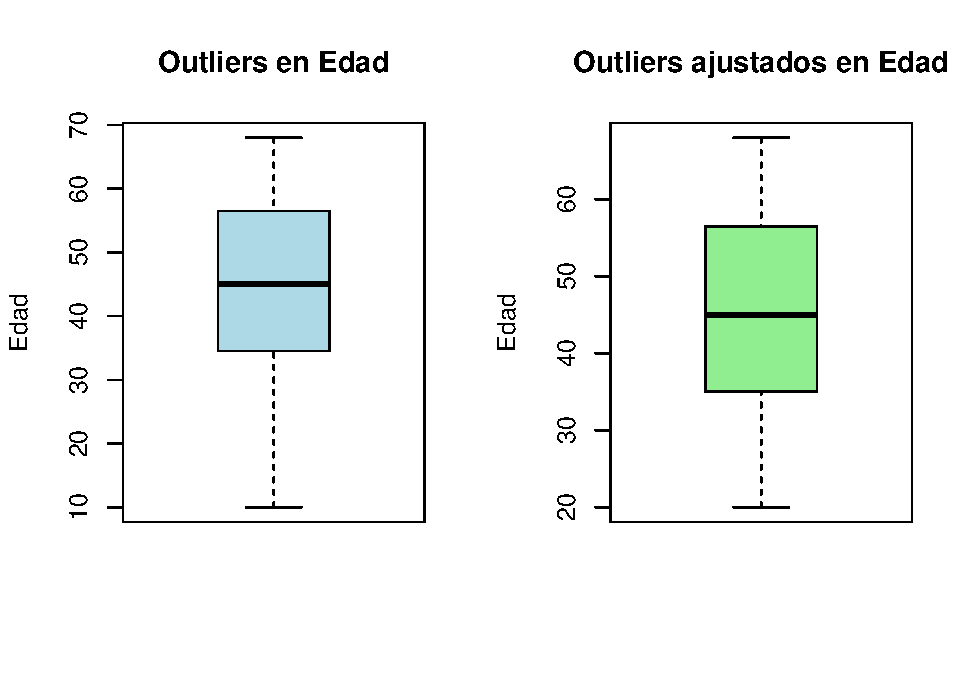
\includegraphics[keepaspectratio]{Reporte01-autors_files/figure-latex/tratamiento_datos_edad-1.pdf}}

\begin{Shaded}
\begin{Highlighting}[]
\CommentTok{\# Restaurar configuración gráfica a 1 gráfico por figura (opcional)}
\FunctionTok{par}\NormalTok{(}\AttributeTok{mfrow =} \FunctionTok{c}\NormalTok{(}\DecValTok{1}\NormalTok{, }\DecValTok{1}\NormalTok{))}
\CommentTok{\#outliers \textless{}{-} boxplot.stats(datos\_base$EDAD)$out ? No funciono }
\end{Highlighting}
\end{Shaded}

\begin{enumerate}
\def\labelenumi{\alph{enumi}.}
\setcounter{enumi}{2}
\tightlist
\item
  Realizar un histograma de la variable edad y describir qué patrones se
  observan entre los clientes (ej. ¿son jóvenes? ¿predomina alguna
  franja de edad?)
\end{enumerate}

\textbf{Rta: } - La franja de edad en la que se presentan mayor numero
de clientes de concesionario estan en la edad de los 40 a los 45 años. -
La franja de 55 a 65 años presenta una gran numeros de clientes - El
sector joven no presenta una alta concentracion con excepcion de la
franja de los 25-30 años

\begin{Shaded}
\begin{Highlighting}[]
\CommentTok{\# Histograma con curva de densidad para la variable EDAD}

\FunctionTok{ggplot}\NormalTok{(datos\_base, }\FunctionTok{aes}\NormalTok{(}\AttributeTok{x =}\NormalTok{ EDAD)) }\SpecialCharTok{+}
  \FunctionTok{geom\_histogram}\NormalTok{(}\AttributeTok{binwidth =} \DecValTok{5}\NormalTok{,}
                 \AttributeTok{fill =} \StringTok{"skyblue"}\NormalTok{,}
                 \AttributeTok{color =} \StringTok{"white"}\NormalTok{,}
                 \AttributeTok{boundary =} \DecValTok{0}\NormalTok{) }\SpecialCharTok{+}

  \CommentTok{\# Añadir línea de densidad}
  \FunctionTok{geom\_density}\NormalTok{(}\FunctionTok{aes}\NormalTok{(}\AttributeTok{y =} \FunctionTok{after\_stat}\NormalTok{(count) }\SpecialCharTok{*} \DecValTok{5}\NormalTok{), }
               \AttributeTok{color =} \StringTok{"red"}\NormalTok{, }
               \AttributeTok{linewidth =} \DecValTok{1}\NormalTok{) }\SpecialCharTok{+}
  \FunctionTok{labs}\NormalTok{(}\AttributeTok{title =} \StringTok{"Distribución de Edades"}\NormalTok{,}
       \AttributeTok{subtitle =} \StringTok{"Histograma con curva de densidad"}\NormalTok{,}
       \AttributeTok{x =} \StringTok{"Edad (años)"}\NormalTok{,}
       \AttributeTok{y =} \StringTok{"Frecuencia"}\NormalTok{,}
       \AttributeTok{caption =} \StringTok{"Ancho de intervalo: 5 años"}\NormalTok{) }\SpecialCharTok{+}
  \CommentTok{\# Ajustar ejes para mejorar la visualización}
  \FunctionTok{scale\_x\_continuous}\NormalTok{(}\AttributeTok{breaks =} \FunctionTok{seq}\NormalTok{(}\DecValTok{0}\NormalTok{, }\FunctionTok{max}\NormalTok{(datos\_base}\SpecialCharTok{$}\NormalTok{EDAD, }\AttributeTok{na.rm =} \ConstantTok{TRUE}\NormalTok{) }\SpecialCharTok{+} \DecValTok{5}\NormalTok{, }\AttributeTok{by =} \DecValTok{5}\NormalTok{)) }\SpecialCharTok{+}
  \FunctionTok{theme\_minimal}\NormalTok{() }\SpecialCharTok{+}
  \FunctionTok{theme}\NormalTok{(}
    \AttributeTok{plot.title =} \FunctionTok{element\_text}\NormalTok{(}\AttributeTok{face =} \StringTok{"bold"}\NormalTok{, }\AttributeTok{size =} \DecValTok{14}\NormalTok{),}
    \AttributeTok{plot.subtitle =} \FunctionTok{element\_text}\NormalTok{(}\AttributeTok{size =} \DecValTok{12}\NormalTok{),}
    \AttributeTok{axis.title =} \FunctionTok{element\_text}\NormalTok{(}\AttributeTok{face =} \StringTok{"bold"}\NormalTok{)}
\NormalTok{  )}
\end{Highlighting}
\end{Shaded}

\pandocbounded{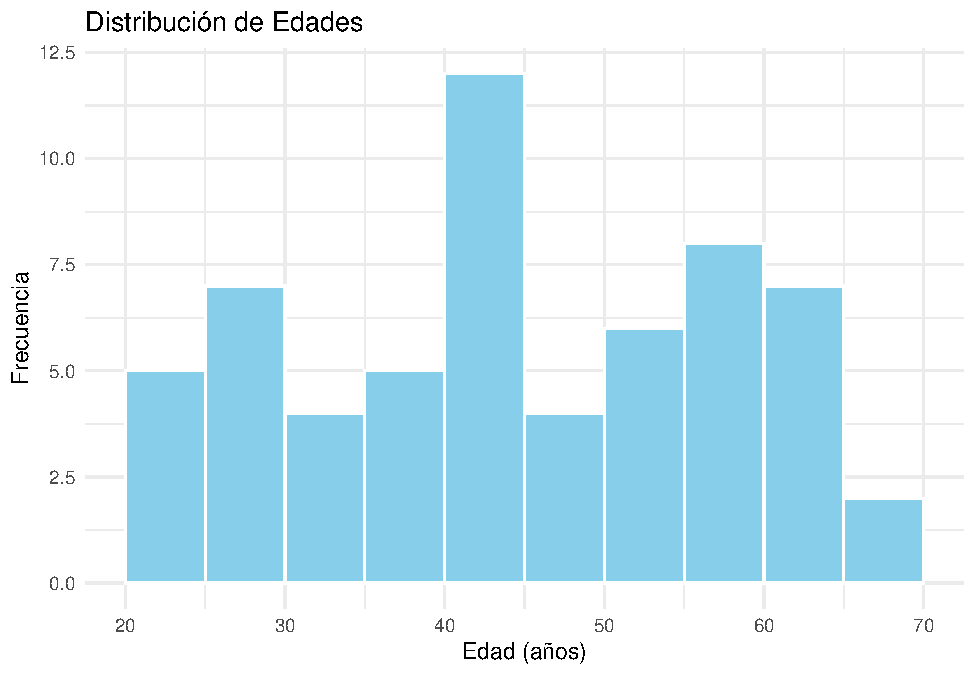
\includegraphics[keepaspectratio]{Reporte01-autors_files/figure-latex/unnamed-chunk-6-1.pdf}}
\newpage

\subsection{5 Análisis de la variable
``Estatura''.}\label{anuxe1lisis-de-la-variable-estatura.}

\begin{enumerate}
\def\labelenumi{\alph{enumi}.}
\tightlist
\item
  Revisar la variable ``ESTATURA'' para asegurar que este correctamente
  importada y limpia. \textbf{Rta:} Se puede observar que la variable
  ESTATURA se encuentra con 60 registros de tipo numeric, sin registros
  de na y con valores ajustados dentro de las estaturas promedio, ya que
  se homologo un valor que se encontraba por fuera del valor posible en
  la edad de una persona.
\end{enumerate}

\begin{Shaded}
\begin{Highlighting}[]
\CommentTok{\#TRATAMIENTO DE DATOS ESTATURA }
\CommentTok{\#Se convierte a numerico el dato caracter}
\NormalTok{datos\_base}\SpecialCharTok{$}\NormalTok{ESTATURA }\OtherTok{\textless{}{-}} \FunctionTok{as.numeric}\NormalTok{(datos\_base}\SpecialCharTok{$}\NormalTok{ESTATURA)}
\CommentTok{\#Datos atipicos}
\NormalTok{rango\_estatura }\OtherTok{\textless{}{-}} \FunctionTok{range}\NormalTok{(datos\_base}\SpecialCharTok{$}\NormalTok{ESTATURA, }\AttributeTok{na.rm =} \ConstantTok{TRUE}\NormalTok{)}
\CommentTok{\# Mostrar dos gráficos uno al lado del otro}
\FunctionTok{par}\NormalTok{(}\AttributeTok{mfrow =} \FunctionTok{c}\NormalTok{(}\DecValTok{1}\NormalTok{, }\DecValTok{2}\NormalTok{))  }\CommentTok{\# 1 fila, 2 columnas}
  \FunctionTok{boxplot}\NormalTok{(datos\_base}\SpecialCharTok{$}\NormalTok{ESTATURA, }
          \AttributeTok{main =} \StringTok{"Outliers en Estatura"}\NormalTok{, }
          \AttributeTok{ylab =} \StringTok{"Estatura"}\NormalTok{, }
          \AttributeTok{col =} \StringTok{"lightblue"}\NormalTok{, }
          \AttributeTok{ylim =}\NormalTok{ rango\_estatura )}
  \CommentTok{\#Se reemplaza el valor especifico de la columna ESTATURA en la persona 31 por la media }
\NormalTok{  media\_sin\_atipicos }\OtherTok{\textless{}{-}} \FunctionTok{median}\NormalTok{(datos\_base}\SpecialCharTok{$}\NormalTok{ESTATURA[datos\_base}\SpecialCharTok{$}\NormalTok{ESTATURA }\SpecialCharTok{!=} \FloatTok{3.5}\NormalTok{], }\AttributeTok{na.rm =} \ConstantTok{TRUE}\NormalTok{)}
\NormalTok{  datos\_base}\SpecialCharTok{$}\NormalTok{ESTATURA[datos\_base}\SpecialCharTok{$}\NormalTok{ESTATURA }\SpecialCharTok{==} \FloatTok{3.450}\NormalTok{] }\OtherTok{\textless{}{-}}\NormalTok{ media\_sin\_atipicos}
\NormalTok{  rango\_estatura }\OtherTok{\textless{}{-}} \FunctionTok{range}\NormalTok{(datos\_base}\SpecialCharTok{$}\NormalTok{ESTATURA, }\AttributeTok{na.rm =} \ConstantTok{TRUE}\NormalTok{)}
  \FunctionTok{boxplot}\NormalTok{(datos\_base}\SpecialCharTok{$}\NormalTok{ESTATURA, }
          \AttributeTok{main =} \StringTok{"Outliers ajustados en ESTATURA"}\NormalTok{,}
          \AttributeTok{ylab =} \StringTok{"Estatura"}\NormalTok{, }\AttributeTok{col =} \StringTok{"lightgreen"}\NormalTok{, }\AttributeTok{ylim =}\NormalTok{rango\_estatura)}
\end{Highlighting}
\end{Shaded}

\pandocbounded{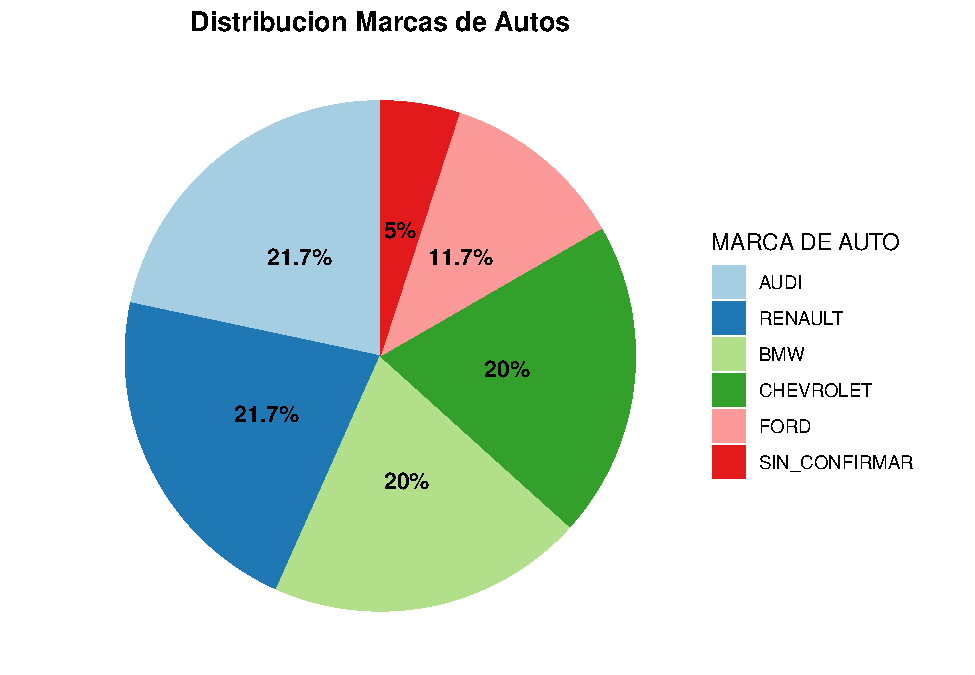
\includegraphics[keepaspectratio]{Reporte01-autors_files/figure-latex/unnamed-chunk-7-1.pdf}}

\begin{Shaded}
\begin{Highlighting}[]
  \CommentTok{\# Restaurar configuración gráfica a 1 gráfico por figura (opcional)}
\FunctionTok{par}\NormalTok{(}\AttributeTok{mfrow =} \FunctionTok{c}\NormalTok{(}\DecValTok{1}\NormalTok{, }\DecValTok{1}\NormalTok{))}
\end{Highlighting}
\end{Shaded}

\begin{Shaded}
\begin{Highlighting}[]
\CommentTok{\#confirmación del tipo de dato}
\FunctionTok{class}\NormalTok{(datos\_base}\SpecialCharTok{$}\NormalTok{ESTATURA)}
\end{Highlighting}
\end{Shaded}

\begin{verbatim}
## [1] "numeric"
\end{verbatim}

\begin{Shaded}
\begin{Highlighting}[]
\CommentTok{\#Se confirma que no tiene na}
\FunctionTok{sum}\NormalTok{(}\FunctionTok{is.na}\NormalTok{(datos\_base}\SpecialCharTok{$}\NormalTok{ESTATURA))}
\end{Highlighting}
\end{Shaded}

\begin{verbatim}
## [1] 0
\end{verbatim}

\begin{Shaded}
\begin{Highlighting}[]
\CommentTok{\#Se confirma estructura y media de la variable}
\FunctionTok{summary}\NormalTok{(datos\_base}\SpecialCharTok{$}\NormalTok{ESTATURA)}
\end{Highlighting}
\end{Shaded}

\begin{verbatim}
##    Min. 1st Qu.  Median    Mean 3rd Qu.    Max. 
##   1.490   1.540   1.650   1.655   1.760   1.810
\end{verbatim}

\begin{enumerate}
\def\labelenumi{\alph{enumi}.}
\setcounter{enumi}{1}
\item
  Identificar los datos faltantes o valores inconsistentes. Eliminar
  esos registros. \textbf{Rta:} En el anterior respuesta se evidencia
  que se identifico el registro de un dato atipico con valor de 3.450 en
  estatura, y se homologo por el valor de la media de los registros
  1,685
\item
  Generar un poligono de frecuencia y una ojiva para analizar la
  distribución de la estatura de los clientes y extraer conclusiones.
  \textbf{Rta:}
\end{enumerate}

\begin{Shaded}
\begin{Highlighting}[]
\FunctionTok{print}\NormalTok{(datos\_base}\SpecialCharTok{$}\NormalTok{ESTATURA)}
\end{Highlighting}
\end{Shaded}

\begin{verbatim}
##  [1] 1.54 1.55 1.60 1.70 1.71 1.80 1.54 1.52 1.51 1.65 1.78 1.76 1.65 1.73 1.71
## [16] 1.80 1.81 1.60 1.51 1.52 1.63 1.76 1.79 1.54 1.78 1.59 1.57 1.60 1.54 1.52
## [31] 1.65 1.52 1.50 1.68 1.78 1.60 1.68 1.80 1.78 1.65 1.71 1.80 1.53 1.52 1.50
## [46] 1.65 1.78 1.76 1.65 1.73 1.71 1.80 1.81 1.49 1.54 1.58 1.60 1.70 1.71 1.80
\end{verbatim}

\begin{Shaded}
\begin{Highlighting}[]
\CommentTok{\#Polígono de frencuencias (sencillo)}

\CommentTok{\# Polígono de frecuencias con intervalos automáticos}
\FunctionTok{ggplot}\NormalTok{(datos\_base, }\FunctionTok{aes}\NormalTok{(}\AttributeTok{x =}\NormalTok{ ESTATURA)) }\SpecialCharTok{+}
  \FunctionTok{geom\_freqpoly}\NormalTok{(}\AttributeTok{binwidth =} \DecValTok{5}\NormalTok{, }\AttributeTok{color =} \StringTok{"steelblue"}\NormalTok{, }\AttributeTok{size =} \DecValTok{1}\NormalTok{) }\SpecialCharTok{+}
  \FunctionTok{labs}\NormalTok{(}\AttributeTok{title =} \StringTok{"Polígono de Frecuencias {-} Estatura"}\NormalTok{,}
       \AttributeTok{x =} \StringTok{"Estatura (metros)"}\NormalTok{,}
       \AttributeTok{y =} \StringTok{"Frecuencia"}\NormalTok{) }\SpecialCharTok{+}
  \FunctionTok{theme\_minimal}\NormalTok{()}
\end{Highlighting}
\end{Shaded}

\begin{verbatim}
## Warning: Using `size` aesthetic for lines was deprecated in ggplot2 3.4.0.
## i Please use `linewidth` instead.
## This warning is displayed once every 8 hours.
## Call `lifecycle::last_lifecycle_warnings()` to see where this warning was
## generated.
\end{verbatim}

\pandocbounded{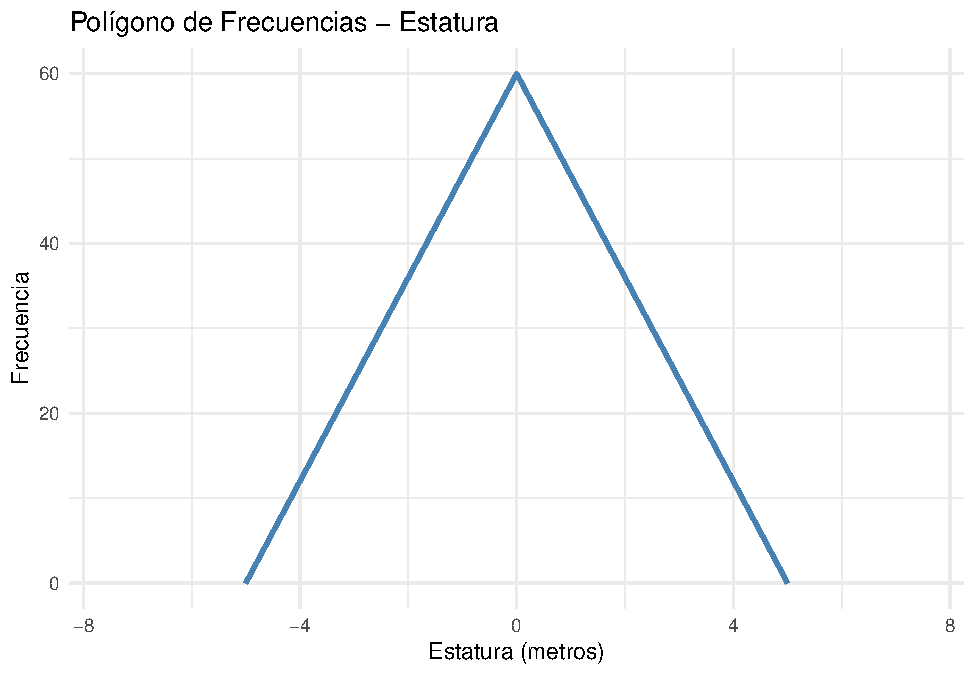
\includegraphics[keepaspectratio]{Reporte01-autors_files/figure-latex/unnamed-chunk-9-1.pdf}}

\begin{Shaded}
\begin{Highlighting}[]
\FunctionTok{summary}\NormalTok{(datos\_base}\SpecialCharTok{$}\NormalTok{EDAD)}
\end{Highlighting}
\end{Shaded}

\begin{verbatim}
##    Min. 1st Qu.  Median    Mean 3rd Qu.    Max. 
##   20.00   35.00   45.00   44.83   56.25   68.00
\end{verbatim}

\begin{Shaded}
\begin{Highlighting}[]
\NormalTok{datos\_base}\SpecialCharTok{$}\NormalTok{EDAD }\OtherTok{\textless{}{-}} \FunctionTok{as.numeric}\NormalTok{(datos\_base}\SpecialCharTok{$}\NormalTok{EDAD)}
\FunctionTok{is.na}\NormalTok{(datos\_base}\SpecialCharTok{$}\NormalTok{EDAD)}
\end{Highlighting}
\end{Shaded}

\begin{verbatim}
##  [1] FALSE FALSE FALSE FALSE FALSE FALSE FALSE FALSE FALSE FALSE FALSE FALSE
## [13] FALSE FALSE FALSE FALSE FALSE FALSE FALSE FALSE FALSE FALSE FALSE FALSE
## [25] FALSE FALSE FALSE FALSE FALSE FALSE FALSE FALSE FALSE FALSE FALSE FALSE
## [37] FALSE FALSE FALSE FALSE FALSE FALSE FALSE FALSE FALSE FALSE FALSE FALSE
## [49] FALSE FALSE FALSE FALSE FALSE FALSE FALSE FALSE FALSE FALSE FALSE FALSE
\end{verbatim}

\begin{Shaded}
\begin{Highlighting}[]
\CommentTok{\# Polígono de frecuencias con intervalos automáticos}
\FunctionTok{ggplot}\NormalTok{(datos\_base, }\FunctionTok{aes}\NormalTok{(}\AttributeTok{x =}\NormalTok{ EDAD)) }\SpecialCharTok{+}
  \FunctionTok{geom\_freqpoly}\NormalTok{(}\AttributeTok{binwidth =} \DecValTok{5}\NormalTok{, }\AttributeTok{color =} \StringTok{"steelblue"}\NormalTok{, }\AttributeTok{size =} \DecValTok{1}\NormalTok{) }\SpecialCharTok{+}
  \FunctionTok{labs}\NormalTok{(}\AttributeTok{title =} \StringTok{"Polígono de Frecuencias {-} Estatura"}\NormalTok{,}
       \AttributeTok{x =} \StringTok{"Estatura (metros)"}\NormalTok{,}
       \AttributeTok{y =} \StringTok{"Frecuencia"}\NormalTok{) }\SpecialCharTok{+}
  \FunctionTok{theme\_minimal}\NormalTok{()}
\end{Highlighting}
\end{Shaded}

\pandocbounded{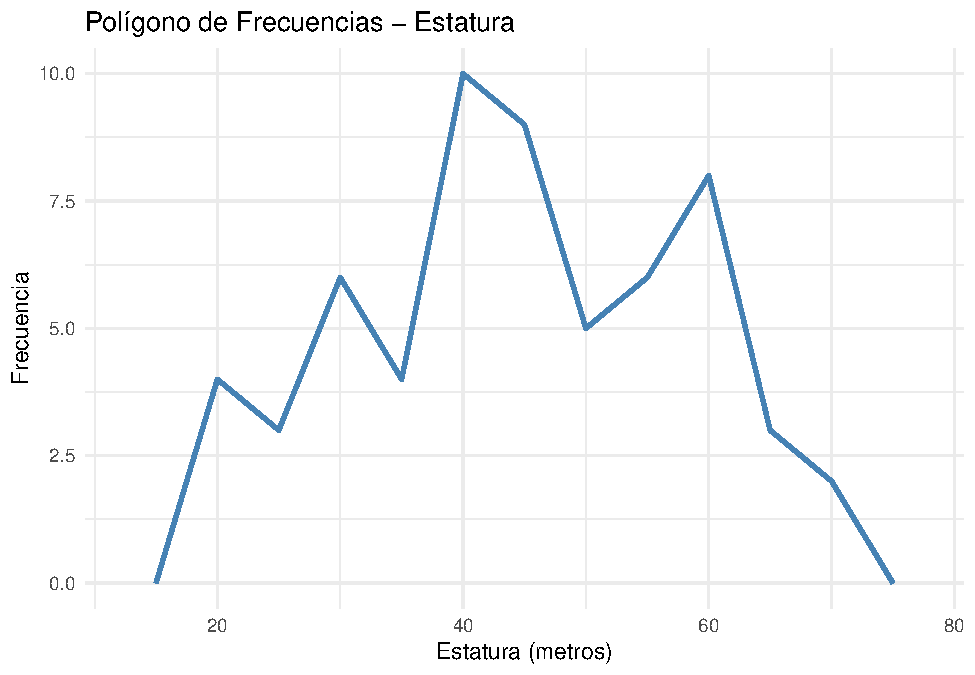
\includegraphics[keepaspectratio]{Reporte01-autors_files/figure-latex/unnamed-chunk-9-2.pdf}}

\begin{Shaded}
\begin{Highlighting}[]
\CommentTok{\#Polígono de frecuencias detallado por intervalos }

\CommentTok{\# Crear intervalos para Estatura}
\CommentTok{\#intervalos\_estatura \textless{}{-} seq(from = floor(min(datos\_base$ESTATURA, na.rm = TRUE)/5)*5,}
\CommentTok{\#                       to = ceiling(max(datos\_base$ESTATURA, na.rm = TRUE)/5)*5,}
\CommentTok{\#                       by = 5)\textasciigrave{}\textasciigrave{}\textasciigrave{}\{r\}}
\CommentTok{\#                       print(intervalos\_estatura)}



\CommentTok{\# Extraer los valores medios de cada intervalo para el eje X}
\CommentTok{\#tabla\_freq\_edad$Valor\_Medio \textless{}{-} as.numeric(sapply(tabla\_freq\_edad$Grupo\_Edad, function(x) \{}
\CommentTok{\#  rango \textless{}{-} as.character(x)}
\CommentTok{\#  limites \textless{}{-} as.numeric(unlist(strsplit(gsub("\textbackslash{}\textbackslash{}[|\textbackslash{}\textbackslash{})|\textbackslash{}\textbackslash{}[|\textbackslash{}\textbackslash{}]", "", rango), ",")))}
\CommentTok{\#  return(mean(limites))}
\CommentTok{\#\}))}

\CommentTok{\#Crear polígono de frecuencias}
\CommentTok{\# ggplot(tabla\_freq\_edad, aes(x = Valor\_Medio, y = Frecuencia, group = 1)) +}
\CommentTok{\#   geom\_point(size = 3, color = "steelblue") +}
\CommentTok{\#   geom\_line(color = "steelblue", size = 1) +}
\CommentTok{\#   geom\_text(aes(label = Frecuencia), vjust = {-}0.8, size = 3.5) +}
\CommentTok{\#   labs(title = "Polígono de Frecuencias {-} Edad por Grupos",}
\CommentTok{\#        x = "Edad (años)",}
\CommentTok{\#        y = "Frecuencia") +}
\CommentTok{\#   scale\_x\_continuous(breaks = tabla\_freq\_edad$Valor\_Medio,}
\CommentTok{\#                      labels = as.character(tabla\_freq\_edad$Grupo\_Edad)) +}
\CommentTok{\#   theme\_minimal() +}
\CommentTok{\#   theme(axis.text.x = element\_text(angle = 45, hjust = 1))}
\CommentTok{\#   }
\CommentTok{\#   OJIVA }
\CommentTok{\#Ojiva de frencuencias acumuladas}

\CommentTok{\# Crear intervalos y calcular frecuencias acumuladas en un solo paso}
\CommentTok{\#histData \textless{}{-} hist(datos\_base$ESTATURA, breaks = seq(min(datos\_base$ESTATURA, na.rm = TRUE), }
\CommentTok{\#                                         max(datos\_base$ESTATURA, na.rm = TRUE) + 5, }
\CommentTok{\#                                         by = 5), }
\CommentTok{\#                plot = FALSE)}

\CommentTok{\# Crear dataframe para la ojiva}
\CommentTok{\#ojiva\_data \textless{}{-} data.frame(}
\CommentTok{\#  x = histData$breaks,}
\CommentTok{\#  y = c(0, cumsum(histData$counts))}
\CommentTok{\#)}

\CommentTok{\# Graficar ojiva}
\CommentTok{\#ggplot(ojiva\_data, aes(x = x, y = y)) +}
\CommentTok{\#  geom\_line(color = "darkred", size = 1) +}
\CommentTok{\#  geom\_point(color = "darkred", size = 3) +}
\CommentTok{\#  labs(title = "Ojiva {-} Frecuencias Acumuladas de Estatura",}
\CommentTok{\#       x = "Estatura (metros)",}
\CommentTok{\#       y = "Frecuencia Acumulada") +}
\CommentTok{\#  theme\_minimal()}
\CommentTok{\#print(datos\_base)}
\end{Highlighting}
\end{Shaded}

\newpage

\subsection{6 Análisis de la variable ``Numero de
hijos''.}\label{anuxe1lisis-de-la-variable-numero-de-hijos.}

\begin{enumerate}
\def\labelenumi{\alph{enumi}.}
\tightlist
\item
  Cambiar el nombre de la varaible a ``n.hijos'' para facilitar su
  manejo. \textbf{Rta:} Se realiza consulta de lal data frame original,
  posteriormente se le aplica el tratamiento solicitado guardando el
  resultado en un nuevo dataframe y por ultimo se consulta el dataframe
  creado para evidenciar el resultado.
\end{enumerate}

\begin{Shaded}
\begin{Highlighting}[]
\FunctionTok{print}\NormalTok{(datos\_base)}
\end{Highlighting}
\end{Shaded}

\begin{verbatim}
## # A tibble: 60 x 9
##    PERSONA     EDAD SEXO  ESTATURA `NIVEL ESCOLAR` `MARCA DE AUTO`
##    <chr>      <dbl> <chr>    <dbl> <chr>           <chr>          
##  1 PERSONA 1     21 M         1.54 MAESTRÍA        AUDI           
##  2 PERSONA 2     26 F         1.55 PROFESIONAL     RENAULT        
##  3 PERSONA 3     30 F         1.6  DOCTORADO       BMW            
##  4 PERSONA 4     31 f         1.7  PROFESIONAL     RENAULT        
##  5 PERSONA 5     35 M         1.71 MAESTRÍA        AUDI           
##  6 PERSONA 6     65 M         1.8  MAESTRÍA        AUDI           
##  7 PERSONA 7     45 M         1.54 MAESTRÍA        BMW            
##  8 PERSONA 8     42 F         1.52 PROFESIONAL     RENAULT        
##  9 PERSONA 9     52 F         1.51 DOCTORADO       RENAULT        
## 10 PERSONA 10    63 M         1.65 DOCTORADO       RENAULT        
## # i 50 more rows
## # i 3 more variables: `NUMERO DE HIJOS` <chr>, SALARIO <dbl>, MASCOTA <chr>
\end{verbatim}

\begin{Shaded}
\begin{Highlighting}[]
\NormalTok{nueva\_datos\_base }\OtherTok{\textless{}{-}}
  \FunctionTok{rename}\NormalTok{(datos\_base,}\AttributeTok{N\_HIJOS=}\StringTok{"NUMERO DE HIJOS"}\NormalTok{)}
\FunctionTok{print}\NormalTok{(nueva\_datos\_base)}
\end{Highlighting}
\end{Shaded}

\begin{verbatim}
## # A tibble: 60 x 9
##    PERSONA   EDAD SEXO  ESTATURA `NIVEL ESCOLAR` `MARCA DE AUTO` N_HIJOS SALARIO
##    <chr>    <dbl> <chr>    <dbl> <chr>           <chr>           <chr>     <dbl>
##  1 PERSONA~    21 M         1.54 MAESTRÍA        AUDI            0       1200000
##  2 PERSONA~    26 F         1.55 PROFESIONAL     RENAULT         5       1250000
##  3 PERSONA~    30 F         1.6  DOCTORADO       BMW             2        900000
##  4 PERSONA~    31 f         1.7  PROFESIONAL     RENAULT         2        800000
##  5 PERSONA~    35 M         1.71 MAESTRÍA        AUDI            1        950000
##  6 PERSONA~    65 M         1.8  MAESTRÍA        AUDI            1       2000000
##  7 PERSONA~    45 M         1.54 MAESTRÍA        BMW             1       2500000
##  8 PERSONA~    42 F         1.52 PROFESIONAL     RENAULT         1       3500000
##  9 PERSONA~    52 F         1.51 DOCTORADO       RENAULT         0       4700000
## 10 PERSONA~    63 M         1.65 DOCTORADO       RENAULT         0       5000000
## # i 50 more rows
## # i 1 more variable: MASCOTA <chr>
\end{verbatim}

\begin{enumerate}
\def\labelenumi{\alph{enumi}.}
\setcounter{enumi}{1}
\tightlist
\item
  Identificar problemas con los datos y eliminar valores inconsistentes.
  \textbf{Rta:} Se identifica que la persona 24 tiene NA en la variable
  hijos, por lo que le aplica el tratamiento y se iguala a 0
\end{enumerate}

\begin{Shaded}
\begin{Highlighting}[]
\FunctionTok{Sys.setlocale}\NormalTok{(}\StringTok{"LC\_ALL"}\NormalTok{, }\StringTok{"es\_CO.UTF{-}8"}\NormalTok{) }
\end{Highlighting}
\end{Shaded}

\begin{verbatim}
## [1] "LC_COLLATE=es_CO.UTF-8;LC_CTYPE=es_CO.UTF-8;LC_MONETARY=es_CO.UTF-8;LC_NUMERIC=C;LC_TIME=es_CO.UTF-8"
\end{verbatim}

\begin{Shaded}
\begin{Highlighting}[]
\CommentTok{\#Se identificarn problemas }
\NormalTok{datos\_base[}\FunctionTok{is.na}\NormalTok{(datos\_base}\SpecialCharTok{$}\StringTok{\textasciigrave{}}\AttributeTok{NUMERO DE HIJOS}\StringTok{\textasciigrave{}}\NormalTok{) }\SpecialCharTok{|} 
\NormalTok{           datos\_base}\SpecialCharTok{$}\StringTok{\textasciigrave{}}\AttributeTok{NUMERO DE HIJOS}\StringTok{\textasciigrave{}} \SpecialCharTok{==} \StringTok{"NA"}\NormalTok{, }
           \FunctionTok{c}\NormalTok{(}\StringTok{"PERSONA"}\NormalTok{, }\StringTok{"NUMERO DE HIJOS"}\NormalTok{)]}
\end{Highlighting}
\end{Shaded}

\begin{verbatim}
## # A tibble: 2 x 2
##   PERSONA    `NUMERO DE HIJOS`
##   <chr>      <chr>            
## 1 PERSONA 21 <NA>             
## 2 PERSONA 24 NA
\end{verbatim}

\begin{Shaded}
\begin{Highlighting}[]
\FunctionTok{print}\NormalTok{(nueva\_datos\_base)}
\end{Highlighting}
\end{Shaded}

\begin{verbatim}
## # A tibble: 60 x 9
##    PERSONA   EDAD SEXO  ESTATURA `NIVEL ESCOLAR` `MARCA DE AUTO` N_HIJOS SALARIO
##    <chr>    <dbl> <chr>    <dbl> <chr>           <chr>           <chr>     <dbl>
##  1 PERSONA~    21 M         1.54 MAESTRÍA        AUDI            0       1200000
##  2 PERSONA~    26 F         1.55 PROFESIONAL     RENAULT         5       1250000
##  3 PERSONA~    30 F         1.6  DOCTORADO       BMW             2        900000
##  4 PERSONA~    31 f         1.7  PROFESIONAL     RENAULT         2        800000
##  5 PERSONA~    35 M         1.71 MAESTRÍA        AUDI            1        950000
##  6 PERSONA~    65 M         1.8  MAESTRÍA        AUDI            1       2000000
##  7 PERSONA~    45 M         1.54 MAESTRÍA        BMW             1       2500000
##  8 PERSONA~    42 F         1.52 PROFESIONAL     RENAULT         1       3500000
##  9 PERSONA~    52 F         1.51 DOCTORADO       RENAULT         0       4700000
## 10 PERSONA~    63 M         1.65 DOCTORADO       RENAULT         0       5000000
## # i 50 more rows
## # i 1 more variable: MASCOTA <chr>
\end{verbatim}

\begin{Shaded}
\begin{Highlighting}[]
\CommentTok{\# Se identifica que la persona 24 tiene NA en la variable hijos, }
\CommentTok{\#por lo que le aplica el tratamiento y se iguala a 0}
\NormalTok{nueva\_datos\_base}\SpecialCharTok{$}\NormalTok{N\_HIJOS[}\FunctionTok{is.na}\NormalTok{(nueva\_datos\_base}\SpecialCharTok{$}\NormalTok{N\_HIJOS) }\SpecialCharTok{|} 
\NormalTok{                               nueva\_datos\_base}\SpecialCharTok{$}\NormalTok{N\_HIJOS }\SpecialCharTok{==} \StringTok{"NA"}\NormalTok{] }\OtherTok{\textless{}{-}} \StringTok{"0"}
\end{Highlighting}
\end{Shaded}

\begin{enumerate}
\def\labelenumi{\alph{enumi}.}
\setcounter{enumi}{2}
\tightlist
\item
  Generar una grafica de barras con colores y analizar que se puede
  concluir sobre el numero de hijos de los clientes. \textbf{Rta:}
\end{enumerate}

\begin{Shaded}
\begin{Highlighting}[]
\NormalTok{tabla\_frecuencias\_hijos }\OtherTok{\textless{}{-}} \FunctionTok{as.data.frame}\NormalTok{(}\FunctionTok{table}\NormalTok{(nueva\_datos\_base}\SpecialCharTok{$}\NormalTok{N\_HIJOS))}
\FunctionTok{names}\NormalTok{(tabla\_frecuencias\_hijos) }\OtherTok{\textless{}{-}} \FunctionTok{c}\NormalTok{(}\StringTok{"N\_HIJOS"}\NormalTok{, }\StringTok{"Frecuencia"}\NormalTok{)}
\CommentTok{\#Organizar Mayor a menor}
\NormalTok{tabla\_frecuencias\_hijos }\OtherTok{\textless{}{-}}\NormalTok{ tabla\_frecuencias\_hijos }\SpecialCharTok{\%\textgreater{}\%} \FunctionTok{arrange}\NormalTok{(}\FunctionTok{desc}\NormalTok{(Frecuencia))}

\CommentTok{\# Gráfico de barras}
\FunctionTok{ggplot}\NormalTok{(tabla\_frecuencias\_hijos, }
       \FunctionTok{aes}\NormalTok{(}\AttributeTok{x =} \FunctionTok{fct\_reorder}\NormalTok{(}\StringTok{\textasciigrave{}}\AttributeTok{N\_HIJOS}\StringTok{\textasciigrave{}}\NormalTok{, Frecuencia, }\AttributeTok{.desc =} \ConstantTok{TRUE}\NormalTok{), }
           \AttributeTok{y =}\NormalTok{ Frecuencia,}
           \AttributeTok{fill =} \StringTok{\textasciigrave{}}\AttributeTok{N\_HIJOS}\StringTok{\textasciigrave{}}\NormalTok{)) }\SpecialCharTok{+}  \CommentTok{\# \textless{}{-} Aquí se asigna color por categoría}
  \FunctionTok{geom\_bar}\NormalTok{(}\AttributeTok{stat =} \StringTok{"identity"}\NormalTok{) }\SpecialCharTok{+}
  \FunctionTok{geom\_text}\NormalTok{(}\FunctionTok{aes}\NormalTok{(}\AttributeTok{label =}\NormalTok{ Frecuencia), }\AttributeTok{vjust =} \SpecialCharTok{{-}}\FloatTok{0.5}\NormalTok{, }\AttributeTok{size =} \FloatTok{3.0}\NormalTok{) }\SpecialCharTok{+}
  \FunctionTok{labs}\NormalTok{(}\AttributeTok{title =} \StringTok{"Dist numero hijos"}\NormalTok{,}
       \AttributeTok{x =} \StringTok{"Numero hijos"}\NormalTok{,}
       \AttributeTok{y =} \StringTok{"Frecuencia"}\NormalTok{) }\SpecialCharTok{+}
  \FunctionTok{scale\_fill\_brewer}\NormalTok{(}\AttributeTok{palette =} \StringTok{"Set3"}\NormalTok{) }\SpecialCharTok{+}
  \FunctionTok{theme\_minimal}\NormalTok{() }\SpecialCharTok{+}
  \FunctionTok{theme}\NormalTok{(}
    \AttributeTok{legend.position =} \StringTok{"none"}\NormalTok{,  }\CommentTok{\# O "bottom" si deseas mostrarla}
    \AttributeTok{axis.text.x =} \FunctionTok{element\_text}\NormalTok{(}\AttributeTok{angle =} \DecValTok{45}\NormalTok{, }\AttributeTok{hjust =} \DecValTok{1}\NormalTok{), }
    \AttributeTok{plot.title =} \FunctionTok{element\_text}\NormalTok{(}\AttributeTok{hjust =} \FloatTok{0.5}\NormalTok{, }\AttributeTok{face =} \StringTok{"bold"}\NormalTok{)}
\NormalTok{  ) }\SpecialCharTok{+}
  \FunctionTok{scale\_y\_continuous}\NormalTok{(}\AttributeTok{expand =} \FunctionTok{expansion}\NormalTok{(}\AttributeTok{mult =} \FunctionTok{c}\NormalTok{(}\DecValTok{0}\NormalTok{, }\FloatTok{0.15}\NormalTok{)))}
\end{Highlighting}
\end{Shaded}

\pandocbounded{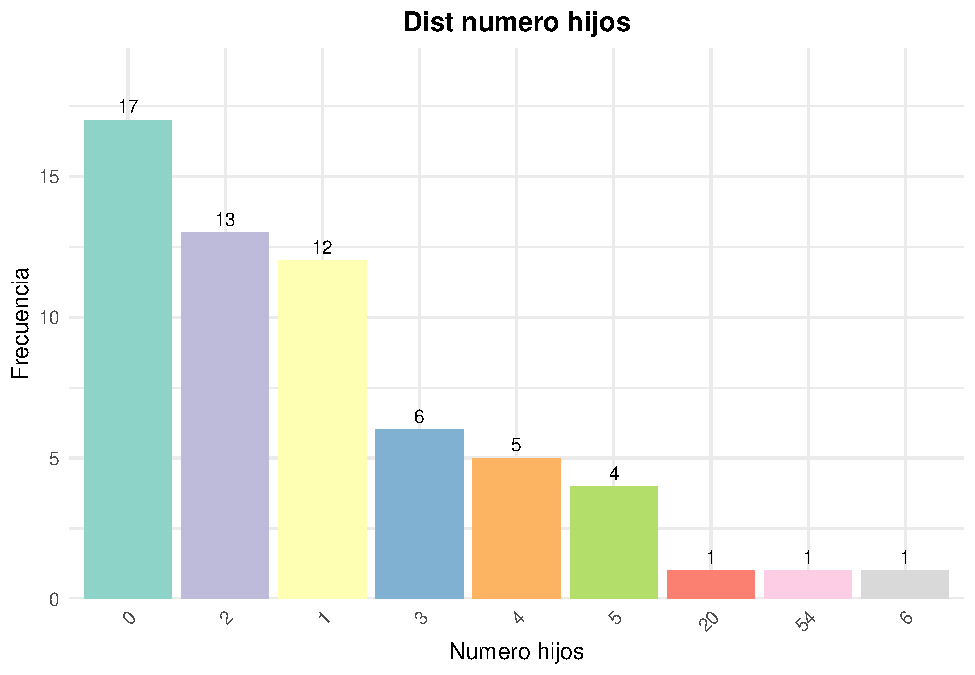
\includegraphics[keepaspectratio]{Reporte01-autors_files/figure-latex/unnamed-chunk-13-1.pdf}}

\newpage

\subsection{7 Análisis de la variable
``Sexo''.}\label{anuxe1lisis-de-la-variable-sexo.}

\begin{enumerate}
\def\labelenumi{\alph{enumi}.}
\tightlist
\item
  Revisar la consistencia de los datos de la varaible ``SEXO'' y
  realizar correcciones en caso de encontrar valores inusuales o
  inconsistentes. \textbf{Rta:}
\end{enumerate}

\begin{Shaded}
\begin{Highlighting}[]
\FunctionTok{is.na}\NormalTok{(datos\_base}\SpecialCharTok{$}\NormalTok{SEXO)}
\end{Highlighting}
\end{Shaded}

\begin{verbatim}
##  [1] FALSE FALSE FALSE FALSE FALSE FALSE FALSE FALSE FALSE FALSE FALSE FALSE
## [13] FALSE FALSE FALSE FALSE FALSE FALSE FALSE FALSE FALSE FALSE FALSE FALSE
## [25] FALSE FALSE FALSE FALSE FALSE FALSE  TRUE FALSE FALSE FALSE FALSE FALSE
## [37] FALSE FALSE FALSE FALSE FALSE FALSE FALSE FALSE FALSE FALSE FALSE FALSE
## [49] FALSE FALSE FALSE FALSE FALSE FALSE FALSE FALSE FALSE FALSE FALSE FALSE
\end{verbatim}

\begin{Shaded}
\begin{Highlighting}[]
\FunctionTok{print}\NormalTok{(nueva\_datos\_base)}
\end{Highlighting}
\end{Shaded}

\begin{verbatim}
## # A tibble: 60 x 9
##    PERSONA   EDAD SEXO  ESTATURA `NIVEL ESCOLAR` `MARCA DE AUTO` N_HIJOS SALARIO
##    <chr>    <dbl> <chr>    <dbl> <chr>           <chr>           <chr>     <dbl>
##  1 PERSONA~    21 M         1.54 MAESTRÍA        AUDI            0       1200000
##  2 PERSONA~    26 F         1.55 PROFESIONAL     RENAULT         5       1250000
##  3 PERSONA~    30 F         1.6  DOCTORADO       BMW             2        900000
##  4 PERSONA~    31 f         1.7  PROFESIONAL     RENAULT         2        800000
##  5 PERSONA~    35 M         1.71 MAESTRÍA        AUDI            1        950000
##  6 PERSONA~    65 M         1.8  MAESTRÍA        AUDI            1       2000000
##  7 PERSONA~    45 M         1.54 MAESTRÍA        BMW             1       2500000
##  8 PERSONA~    42 F         1.52 PROFESIONAL     RENAULT         1       3500000
##  9 PERSONA~    52 F         1.51 DOCTORADO       RENAULT         0       4700000
## 10 PERSONA~    63 M         1.65 DOCTORADO       RENAULT         0       5000000
## # i 50 more rows
## # i 1 more variable: MASCOTA <chr>
\end{verbatim}

\begin{enumerate}
\def\labelenumi{\alph{enumi}.}
\setcounter{enumi}{1}
\tightlist
\item
  Crea una tabla de frecuencias y extraer conclusiones sobre la
  proporcion de hombres y mujeres en el conjunto de clientes.
  \textbf{Rta:}
\end{enumerate}

\newpage

\subsection{8 Preguntas de
investigación.}\label{preguntas-de-investigaciuxf3n.}

Utilizando las herramientas de RStudio (filtros, agrupaciones etc),
responder a las siguientes preguntas: a. ¿Cuántos clientes tienen
mascota?

\begin{Shaded}
\begin{Highlighting}[]
\NormalTok{no\_clientes\_mascota }\OtherTok{\textless{}{-}}\NormalTok{ datos\_base }\SpecialCharTok{\%\textgreater{}\%}  
  \FunctionTok{filter}\NormalTok{(}\SpecialCharTok{!}\FunctionTok{is.na}\NormalTok{(MASCOTA) }\SpecialCharTok{\&} \FunctionTok{toupper}\NormalTok{(MASCOTA) }\SpecialCharTok{==} \StringTok{"SI"}\NormalTok{) }\SpecialCharTok{\%\textgreater{}\%} 
  \FunctionTok{count}\NormalTok{()}
\CommentTok{\#print(no\_clientes\_mascota)}
\end{Highlighting}
\end{Shaded}

\textbf{Rta: } El numero de clientes que tiene mascota es: \textbf{30}

\begin{enumerate}
\def\labelenumi{\alph{enumi}.}
\setcounter{enumi}{1}
\tightlist
\item
  ¿Cuántos clientes mayores de 25 años tienen una maestría?
\end{enumerate}

\begin{Shaded}
\begin{Highlighting}[]
\NormalTok{no\_clientes\_mayores\_mascota }\OtherTok{\textless{}{-}}\NormalTok{ datos\_base }\SpecialCharTok{\%\textgreater{}\%} 
  \FunctionTok{mutate}\NormalTok{(}\AttributeTok{EDAD =} \FunctionTok{as.numeric}\NormalTok{(EDAD)) }\SpecialCharTok{\%\textgreater{}\%} 
  \FunctionTok{filter}\NormalTok{(}\SpecialCharTok{!}\FunctionTok{is.na}\NormalTok{(EDAD) }\SpecialCharTok{\&}\NormalTok{ EDAD }\SpecialCharTok{\textgreater{}} \DecValTok{25}\NormalTok{) }\SpecialCharTok{\%\textgreater{}\%} 
  \FunctionTok{filter}\NormalTok{( }\StringTok{\textasciigrave{}}\AttributeTok{NIVEL ESCOLAR}\StringTok{\textasciigrave{}} \SpecialCharTok{==} \StringTok{"MAESTRÍA"}\NormalTok{) }\SpecialCharTok{\%\textgreater{}\%}
  \FunctionTok{count}\NormalTok{()}
    \CommentTok{\#select(PERSONA, EDAD, \textasciigrave{}NIVEL ESCOLAR\textasciigrave{})}
\end{Highlighting}
\end{Shaded}

\textbf{Rta: } El numero de clientes mayores a 25 años con maestria son
\textbf{17}

\begin{enumerate}
\def\labelenumi{\alph{enumi}.}
\setcounter{enumi}{2}
\tightlist
\item
  ¿Cuántos clientes con doctorado ganan mas de 2 millones de pesos?
\end{enumerate}

\begin{Shaded}
\begin{Highlighting}[]
\CommentTok{\#print(datos\_base)}
\CommentTok{\#datos\_clientes\_doctorado\textless{}{-} sum(datos\_base$\textasciigrave{}NIVEL ESCOLAR\textasciigrave{} == "DOCTORADO") \%\textgreater{}\% filter(datos\_base$SALARIO\textgreater{}2000000)}
\NormalTok{no\_clientes\_doctorado }\OtherTok{\textless{}{-}}\NormalTok{ datos\_base }\SpecialCharTok{\%\textgreater{}\%} \FunctionTok{filter}\NormalTok{(}\StringTok{\textasciigrave{}}\AttributeTok{NIVEL ESCOLAR}\StringTok{\textasciigrave{}} \SpecialCharTok{==} \StringTok{"DOCTORADO"} \SpecialCharTok{\&}\NormalTok{ SALARIO }\SpecialCharTok{\textgreater{}} \DecValTok{2000000}\NormalTok{) }\SpecialCharTok{\%\textgreater{}\%} \FunctionTok{count}\NormalTok{()}
\end{Highlighting}
\end{Shaded}

\textbf{Rta: } El numero de clientes con doctorado y salario superior a
\$2'000.000 es: 13

\begin{enumerate}
\def\labelenumi{\alph{enumi}.}
\setcounter{enumi}{3}
\tightlist
\item
  ¿Cuál es el promedio de salario por cada categoría de la variable
  ``MARCA DE AUTO''?
\end{enumerate}

\begin{Shaded}
\begin{Highlighting}[]
\NormalTok{salario\_promedio\_por\_marca\_auto }\OtherTok{\textless{}{-}}\NormalTok{ datos\_base }\SpecialCharTok{\%\textgreater{}\%}
  \FunctionTok{group\_by}\NormalTok{(}\StringTok{\textasciigrave{}}\AttributeTok{MARCA DE AUTO}\StringTok{\textasciigrave{}}\NormalTok{) }\SpecialCharTok{\%\textgreater{}\%}
  \FunctionTok{summarise}\NormalTok{(}\AttributeTok{promedio\_salario =} \FunctionTok{mean}\NormalTok{(SALARIO, }\AttributeTok{na.rm =} \ConstantTok{TRUE}\NormalTok{))}
\FunctionTok{kable}\NormalTok{(salario\_promedio\_por\_marca\_auto, }\AttributeTok{caption =} \StringTok{"Promedio de Salario por Marca de Auto"}\NormalTok{) }\SpecialCharTok{\%\textgreater{}\%}
  \FunctionTok{kable\_styling}\NormalTok{(}\AttributeTok{full\_width =} \ConstantTok{FALSE}\NormalTok{, }\AttributeTok{position =} \StringTok{"left"}\NormalTok{)}
\end{Highlighting}
\end{Shaded}

\begin{longtable}[l]{lr}
\caption{\label{tab:unnamed-chunk-17}Promedio de Salario por Marca de Auto}\\
\toprule
MARCA DE AUTO & promedio\_salario\\
\midrule
AUDI & 2226923\\
BMW & 2441667\\
CHEVROLET & 4500000\\
FORD & 5114286\\
RENAULT & 3057692\\
\addlinespace
SIN\_CONFIRMAR & 3133333\\
\bottomrule
\end{longtable}

\begin{Shaded}
\begin{Highlighting}[]
\CommentTok{\#print(salario\_promedio\_por\_marca\_auto)}
\end{Highlighting}
\end{Shaded}


\end{document}
